%% Canonical MTAP manuscript.
%% Build: pdflatex main && bibtex main && pdflatex main && pdflatex main
\documentclass[sn-basic,Numbered]{sn-jnl}

\usepackage{graphicx}
\usepackage{amsmath,amssymb,amsfonts}
\usepackage{booktabs}
\usepackage[table,dvipsnames]{xcolor}
\usepackage{manyfoot}
\usepackage{hyperref}
\hypersetup{bookmarksdepth=2}
\usepackage{tikz}
\usetikzlibrary{arrows.meta,positioning,calc}
\usepackage{enumitem}
\usepackage{array}
\newcolumntype{L}[1]{>{\raggedright\arraybackslash}p{#1}}

\definecolor{headerblue}{HTML}{1B4F72}
\definecolor{rowlight}{HTML}{EDF3F8}
\definecolor{rulegray}{HTML}{9AA5B1}
\definecolor{accentgreen}{HTML}{1E8449}
\definecolor{accentred}{HTML}{C0392B}
\definecolor{accentorange}{HTML}{E67E22}
\definecolor{accentpurple}{HTML}{7D3C98}
\definecolor{catbovw}{HTML}{C2185B}
\newcommand{\hd}[1]{\textcolor{white}{\textbf{#1}}}
\newcommand{\polup}{\ensuremath{\uparrow}}
\newcommand{\poldown}{\ensuremath{\downarrow}}

\begin{document}

\title[Component-level audit of quality scoring]{A Component-Level Audit of
No-Reference Quality Scoring in a Multi-Video Summarization Pipeline}

%% NOTE: confirm author list, ORCIDs and affiliations before submission.
\author*[1]{\fnm{Jader L.} \sur{de Souza Gon\c{c}alves}}\email{jaderlouis@proton.me}
\author[1]{\fnm{Rudinei} \sur{Goularte}}\email{rudinei@icmc.usp.br}
\affil[1]{\orgdiv{Instituto de Ci\^{e}ncias Matem\'{a}ticas e de Computa\c{c}\~{a}o},
  \orgname{Universidade de S\~{a}o Paulo (USP)},
  \orgaddress{\city{S\~{a}o Carlos}, \state{SP}, \country{Brazil}}}

\abstract{A visual-quality criterion in a multi-video summarization pipeline is
implemented with Bag-of-Visual-Words and term frequency--inverse document
frequency, techniques designed for retrieval rather than perceptual assessment.
This study audits that operation while leaving the remaining pipeline stages
unchanged. An exact factorization separates descriptor count from mean IDF weight;
measurements on three image-quality databases and an ablation of 19 extractors
show that descriptor count dominates the evaluated configurations. On 800
paired decisions constructed by degrading the same broadcast content, the
deployed score selects the unmodified member in 65.1\% of cases and reverses
direction under white noise and JPEG compression; LIQE reaches 99.5\%. A dependency-aware
screening protocol retains LIQE, QualiCLIP and CLIP-IQA$+$. The downstream
technical output of DOVER, reserved from screening, reaches 97.6\% accuracy on
the constructed pairs ($[96.1,99.0]$). With the
same ten frames and mean pooling, SIFT+BoVW and LIQE still differ in 16 of 42
clusters, with a positive hierarchical DOVER contrast. Replacing the complete deployed
operation, while holding all other pipeline stages fixed, changes 22 of 42
segments. The DOVER
technical-branch point estimate rises by 25.5 percentage points of the global
achievable range, but its topic-block $[-12.1,+54.9]$ and hierarchical
$[-17.2,+59.6]$ intervals both cross zero. The application therefore establishes
changed decisions, not improved viewer experience or a confirmed population-level
output effect; no human compositional preferences were collected.}

\keywords{Multi-video summarization, No-reference image quality assessment,
Content selection criteria, Benchmark evaluation, Broadcast news video}

\maketitle

\section{Introduction}\label{sec:intro}

Video summarization reduces long audiovisual collections to selected keyframes,
shots or segments~\citep{truong2007video_abstraction,apostolidis2021survey}.
When several sources cover the same topic, selection must also handle
cross-source redundancy~\citep{li2010videommr,panda2017collaborative,
wu2020mvsgcn}. A multi-video pipeline therefore combines several criteria: a
segment can be relevant yet redundant, visually informative yet technically
poor, or temporally misplaced.

HSMVideoSumm makes those criteria inspectable. A study with human summarizers of
multi-source news identified five recurrent strategies---removing introductory
passages, filtering subjective content, detecting redundancy, selecting for
visual quality and ordering chronologically---and implemented them as separate
stages~\citep{barbieri2021content,barbieri2021tese}. The present study concerns
only the fourth stage. Segmentation, subjectivity filtering, redundancy
detection and ordering remain unchanged. Once the pipeline treats segments as a
redundant cluster, visual quality acts as a tie-breaker; this conditional design
does not imply that cluster members have identical semantic utility.

The scientific issue is the distinction between a criterion and the operation
that implements it. The criterion is human-grounded because it was observed in
the summarization study. Its implementation is a later engineering choice:
Scale-Invariant Feature Transform (SIFT) descriptors are quantized through
Bag-of-Visual-Words (BoVW), weighted with term frequency--inverse document
frequency (TF-IDF), and summed~\citep{lowe2004sift,sivic2003videogoogle,
csurka2004bovw,salton1988tfidf}. SIFT, BoVW and TF-IDF were developed for
matching, retrieval and categorization, not for predicting perceptual quality.
Calling their aggregate a quality score does not establish construct validity.

No-reference image quality assessment (NR-IQA) provides alternatives because
segments from different broadcasters have no common undistorted reference. The
available families include natural-scene-statistics, supervised convolutional
and transformer regressors, and vision--language models
~\citep{mittal2012brisque,mittal2013niqe,ke2021musiq,zhang2023liqe,
agnolucci2024qualiclip}. The question is not whether a newer model produces a
higher number, but whether the deployed operation responds to the construct it
names, whether that behaviour can be explained, and whether replacing the
operation changes the pipeline output.

The study makes three contributions. First, it derives an exact factorization
that isolates the descriptor-count and mean-IDF-weight channels of the deployed
score, then measures which channel dominates across image databases, broadcast
segments and 19 convolutional neural network (CNN) extractor substitutions.
Second, it combines human-score
association with within-reference degradation sensitivity and a constructed
experiment containing 800 paired decisions between an unmodified signal and a
deterministically degraded counterpart. Third, it applies a common screening
rule and substitutes the complete visual-quality operation in 42 redundancy
clusters while holding every other pipeline stage fixed, measuring both changed
selections and model-reference scores of the selected segments. Training-database overlap,
detectable-keypoint conditioning, alternative pooling, overlay strata,
predictions recorded in a commit whose metadata predates the experiment and
computational details are auxiliary diagnostics reported in the supplementary
material.

The resulting claim is deliberately bounded: the factorization explains the
observed count dominance and failure of the evaluated BoVW+TF-IDF
configurations. It is not a theorem that every possible visual vocabulary,
normalization or extractor must fail. Likewise, the application study separates
Q-Align, which defines the in-domain screening floor, from DOVER, which is used
only for output sensitivity; neither model substitutes for human preference
judgments.

\section{Related work}\label{sec:related}

\subsection{Quality-aware multi-video summarization}

Extractive summarization selects existing frames or temporal segments, whereas
abstractive approaches generate derived representations
~\citep{truong2007video_abstraction,apostolidis2021survey}. Multi-video methods
add explicit cross-source redundancy and diversity. Video-MMR formalized the
setting~\citep{li2010videommr}; sparse and collaborative formulations improved
diversity across topic-related videos~\citep{panda2017diversity,
panda2017collaborative}; graph models subsequently represented inter-video
relations directly~\citep{wu2020mvsgcn}. These methods address
representativeness, coverage and redundancy, but they do not validate a
visual-quality proxy used to choose between redundant candidates.

HSMVideoSumm instead derived selection criteria from human summarization
practice and implemented each criterion as an explicit pipeline stage
~\citep{barbieri2021content,barbieri2021tese}. This modularity permits a
component-level audit: the same clusters, filters and ordering can be held fixed
while the operation used for visual quality is tested and replaced. The object
of comparison is therefore neither a new summarizer nor an overall benchmark
against SumMe or TVSum; it is one inspectable decision inside a multi-source
news pipeline.

The use of image-quality assessment in summarization is not itself new.
VSQUAL used objective IQA measures for shot-boundary detection, keyframe
extraction and summary construction~\citep{cirne2014vsqual}. Jeong et al. also
combined representativeness with contrast, blur and image-skew measures when
selecting keyframes for static video summaries~\citep{jeong2016static}. The present
contribution is different: it does not claim novelty for adding IQA, but for a
mechanistic construct-validation audit of an already deployed quality operation,
followed by dependency-aware propagation of an operation-level substitution.

\subsection{No-reference quality assessment and transfer}

Image quality assessment predicts perceived degradation. Full-reference
measures require an undistorted original and are unsuitable when candidates come
from different broadcasters~\citep{wang2004ssim,zhai2020iqa_survey}. NR-IQA
instead estimates quality from the test image alone. BRISQUE and NIQE model
departures from natural-scene statistics~\citep{mittal2012brisque,
mittal2013niqe}; DBCNN and HyperIQA learn opinion-supervised convolutional
representations~\citep{zhang2020dbcnn,su2020hyperiqa}; MUSIQ and TOPIQ use
multi-scale or top-down attention~\citep{ke2021musiq,chen2024topiq}.

Vision--language formulations based on Contrastive Language--Image Pre-training
(CLIP) provide a different inductive bias. CLIP-IQA uses
antonym prompts~\citep{wang2023clipiqa}; LIQE jointly predicts quality,
distortion and scene~\citep{zhang2023liqe}; QualiCLIP learns from rankings of
synthetically degraded pairs without opinion scores~\citep{agnolucci2024qualiclip}.
Q-Align maps multimodal-model outputs to discrete quality levels
~\citep{wu2024qalign}. These models differ not only architecturally but also in
their exposure to opinion databases. A result on training data measures fit,
whereas use in a new broadcast domain requires transfer. Cross-database
evaluation is therefore essential, and published work has shown that
in-database NR-IQA performance can overstate generalization
~\citep{pinson2023nrbroadcast,cao2024datacentric}.

KADID-10k supplies controlled synthetic distortions
~\citep{lin2019kadid}; KonIQ-10k and LIVE In the Wild (CLIVE) contain authentic
in-the-wild images~\citep{hosu2020koniq,ghadiyaram2016clive}. Their differences
make them complementary validation settings, but comparisons among unmatched
databases and checkpoints do not identify causal effects of training exposure
or distortion regime. The complete descriptive contrasts are consequently kept
in Supplementary Table~S15 rather than presented as a principal contribution.

Two further cautions affect the broadcast application. First, professional and
user-generated video can contain temporal impairments that a frame-wise image
score cannot observe; video-quality models were developed partly for this reason
~\citep{wang2021uvq,huang2023xgcvqa}. Second, high correlation on a reused
database need not imply difficult pairwise discrimination. Database range and
subjective-score uncertainty affect correlation~\citep{krasula2016methodology},
and recent multimodal benchmarks report that comparative quality judgments can
behave differently from absolute scoring~\citep{zhang2024qbenchplus}. Newer
distributional quality models also exceed earlier reference-model results on
some databases~\citep{you2025deqascore}. Accordingly, Q-Align and DOVER are
treated here as complementary contemporary references, not definitive ground
truth or evidence that temporal modeling itself causes an advantage.

\subsection{The unresolved measurement problem}

SIFT, BoVW and TF-IDF encode local-feature occurrence and rarity for retrieval
~\citep{lowe2004sift,sivic2003videogoogle,csurka2004bovw,
salton1988tfidf}. Spatial Information similarly quantifies scene complexity
rather than perceptual quality~\citep{itu_p910,robitza2021siti}. Such features
may correlate with opinion scores in a particular collection, but correlation
does not show that they measure quality or remain valid under controlled
degradation.

The gap addressed here is narrower than the general problem of quality-aware
summarization. Existing work establishes multi-video selection criteria,
specialized NR-IQA methods and prior use of IQA in summarization, yet the
operation implementing HSMVideoSumm's human-grounded visual-quality criterion
was not validated as a quality measure. This study links a mechanistic analysis
of that operation to external human scores, construction-defined degradation
pairs and a controlled operation-level substitution in the pipeline. That
combination distinguishes construct validation from merely integrating an
available IQA model.

\section{Audit design}\label{sec:method}

The audit combines four forms of evidence (Fig.~\ref{fig:overview}): a
mechanistic analysis of the deployed score, external validation against human
opinion scores, construction-defined degradation pairs in the broadcast domain,
and an operation-level substitution in the summarization pipeline. A method is
eligible only if it responds to controlled degradation, generalizes to every
unseen opinion database and exceeds a reference-model agreement floor in the
deployment domain.

\begin{figure}[!ht]
\centering
\resizebox{\textwidth}{!}{%
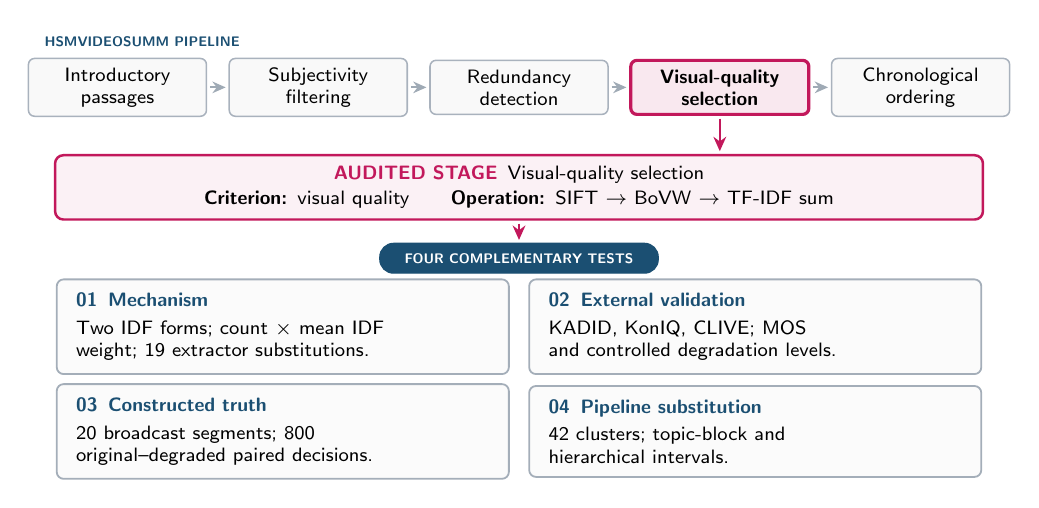
\begin{tikzpicture}[
  stage/.style={rectangle,rounded corners=2.2pt,minimum height=.68cm,
    text width=2.05cm,align=center,font=\sffamily\scriptsize,
    draw=rulegray!85,fill=gray!5,line width=.55pt,inner xsep=3pt},
  focus/.style={stage,draw=catbovw,fill=catbovw!10,line width=1.15pt,
    font=\sffamily\bfseries\scriptsize},
  operation/.style={rectangle,rounded corners=3pt,minimum height=.78cm,
    text width=11.55cm,align=center,font=\sffamily\scriptsize,
    draw=catbovw,fill=catbovw!6,line width=.9pt,inner ysep=4pt},
  audit/.style={rectangle,rounded corners=2.5pt,minimum height=1.05cm,
    text width=5.25cm,align=left,font=\sffamily\scriptsize,
    draw=rulegray!90,fill=gray!3,line width=.65pt,inner xsep=7pt,inner ysep=5pt},
  evidencehead/.style={rectangle,rounded corners=5pt,minimum height=.38cm,
    font=\sffamily\bfseries\tiny,text=white,fill=headerblue,draw=headerblue,
    inner xsep=9pt,inner ysep=2.5pt},
  flow/.style={-{Stealth[length=4.8pt,width=4.2pt]},line width=.65pt,
    draw=rulegray!95,shorten <=1pt,shorten >=1pt},
  focusflow/.style={-{Stealth[length=5.2pt,width=4.6pt]},line width=.9pt,
    draw=catbovw,shorten <=1pt,shorten >=1pt}]

\node[font=\sffamily\bfseries\tiny,text=headerblue,anchor=west]
  at (-6.15,5.05) {HSMVIDEOSUMM PIPELINE};
\node[stage] (a) at (-5.10,4.47) {Introductory\\passages};
\node[stage] (b) at (-2.55,4.47) {Subjectivity\\filtering};
\node[stage] (c) at (0,4.47) {Redundancy\\detection};
\node[focus] (d) at (2.55,4.47) {Visual-quality\\selection};
\node[stage] (e) at (5.10,4.47) {Chronological\\ordering};
\draw[flow] (a.east)--(b.west);
\draw[flow] (b.east)--(c.west);
\draw[flow] (c.east)--(d.west);
\draw[flow] (d.east)--(e.west);

\node[operation] (op) at (0,3.20)
  {\textcolor{catbovw}{\textbf{AUDITED STAGE}}\enspace Visual-quality selection\\[1pt]
   \textbf{Criterion:} visual quality\qquad
   \textbf{Operation:} SIFT $\rightarrow$ BoVW $\rightarrow$ TF-IDF sum};
\draw[focusflow] (d.south)--(d.south |- op.north);

\node[evidencehead] (eh) at (0,2.30) {FOUR COMPLEMENTARY TESTS};
\draw[focusflow] (op.south)--(eh.north);

\node[audit] (m) at (-3.0,1.43)
  {\textcolor{headerblue}{\textbf{01\enspace Mechanism}}\\[2pt]
   Two IDF forms; count $\times$ mean IDF\\weight; 19 extractor substitutions.};
\node[audit] (x) at (3.0,1.43)
  {\textcolor{headerblue}{\textbf{02\enspace External validation}}\\[2pt]
   KADID, KonIQ, CLIVE; MOS\\and controlled degradation levels.};
\node[audit] (g) at (-3.0,.10)
  {\textcolor{headerblue}{\textbf{03\enspace Constructed truth}}\\[2pt]
   20 broadcast segments; 800\\original--degraded paired decisions.};
\node[audit] (p) at (3.0,.10)
  {\textcolor{headerblue}{\textbf{04\enspace Pipeline substitution}}\\[2pt]
   42 clusters; topic-block and\\hierarchical intervals.};
\end{tikzpicture}}
\caption{Scope and evidence flow. Top: the five HSMVideoSumm stages, with
visual-quality selection highlighted. Bottom: four complementary tests of the
operation implementing that criterion. All other pipeline stages remain fixed.}
\label{fig:overview}
\end{figure}

\subsection{Data and units of analysis}\label{sec:data}

The external benchmark uses KADID-10k, KonIQ-10k and LIVE In the Wild (CLIVE).
KADID-10k contains 10,125 distorted images derived from 81 references, with 25
distortion types at five levels and Differential Mean Opinion Scores
(DMOS)~\citep{lin2019kadid}. KonIQ-10k contains 10,073 authentically distorted
images, approximately 1.2 million ratings and Mean Opinion Scores
(MOS)~\citep{hosu2020koniq}; CLIVE
contains 1,162 mobile photographs with authentic distortions
~\citep{ghadiyaram2016clive}. No method is retrained or fine-tuned.

The deployment analysis uses the redundancy stage produced by HSMVideoSumm over
19 of its 21 news topics: 42 multi-member clusters, 93 segment slots and 83
distinct segments. The other two topics contain no multi-member cluster. These
clusters are operational inputs, not proof of equal semantic utility. The
original human redundancy annotations cover only 15 clusters and are retained
as a supplementary sensitivity analysis (Tables~S1, S7, S8 and S11); the
42-cluster set is primary because it is the set encountered by the deployed
pipeline.

Still-image scorers receive frames sampled uniformly at 1 frame per second and
are pooled by the arithmetic mean,
\begin{equation}
S(s)=\frac{1}{n_s}\sum_{i=1}^{n_s}\phi(f_i),
\label{eq:meanpool}
\end{equation}
where $\phi$ is the per-frame score. The deployed operation instead applies its
own key-frame selector, quantizes retained descriptors into a vocabulary of
$K=300$ visual words and sums
\begin{equation}
S_{\mathrm{BoVW}}(s)=\sum_i\sum_{v=1}^{K}
\mathrm{tf}(v,f_i)\,\mathrm{idf}(v).
\label{eq:bovw}
\end{equation}
Sampling, scoring and pooling jointly define the operation occupying the
visual-quality stage, so the primary comparison evaluates complete operations
while holding every other stage fixed. A matched-input control additionally gives
SIFT+BoVW and LIQE the same fixed set of at most ten uniformly spaced 1-fps
frames and arithmetic-mean pooling. For SIFT, common-frame descriptors fit a
seeded per-cluster vocabulary with
$K_{\mathrm{eff}}=\min(300,n_{\mathrm{descriptors}})$; candidate segments are
the documents for the deployed $\log_{10}(K_{\mathrm{eff}}/\mathrm{df})$ IDF.
Empty-descriptor frames remain as zeros in the mean; all observed segments
yielded descriptors and no top-score ties occurred. This isolates scorer
identity within the matched-input regime (Tables~S6, S9 and S11).

\subsection{Scorers, references and polarity}\label{sec:methods}

The complete-case comparison contains the deployed SIFT+BoVW score and ten
NR-IQA candidates: BRISQUE, NIQE, DBCNN, HyperIQA, MUSIQ, TOPIQ, CLIP-IQA,
CLIP-IQA$+$, LIQE and QualiCLIP. Keypoint density, Spatial Information, deep
feature norms and the second IDF formulation are diagnostic controls. A
separate ablation replaces SIFT with 19 convolutional extractors while holding
the vocabulary, weighting and aggregation fixed. ARNIQA and TReS extend
coverage on completed axes but are excluded from complete-case screening;
MANIQA was not completed before the experimental freeze (Table~S13).
Released-weight supervision, checkpoint role,
polarity and GPU requirements are summarized in Table~\ref{tab:methods} and
listed in full in Table~S13~\citep{agnolucci2024arniqa,golestaneh2022tres,
yang2022maniqa}.

\begin{table}[!ht]
\centering
\caption{Scorers needed to interpret the main comparison. Sup.: K = released
KonIQ-10k opinion-trained checkpoint; L = LIVE opinion training; OU = opinion-
unaware; M = multi-database opinion mixture; -- = no opinion data. Polarity is
declared before evaluation. D = deployed, C = candidate, R = reference, X =
diagnostic or ablation. Partial-coverage methods remain outside screening.}
\label{tab:methods}
\scriptsize
\setlength{\tabcolsep}{3.3pt}
\renewcommand{\arraystretch}{1.05}
\begin{tabular}{@{}L{2.2cm}L{2.35cm}L{3.65cm}cccc@{}}
\toprule
\rowcolor{headerblue}
\hd{Method} & \hd{Family} & \hd{Measured construct} & \hd{Sup.} & \hd{Pol.} & \hd{GPU} & \hd{Role} \\
\midrule
\rowcolor{catbovw!12}SIFT+BoVW & handcrafted retrieval & TF-IDF-weighted visual-word count & -- & \polup & no & D \\
Keypoint density & handcrafted & detectable keypoints per frame & -- & \polup & no & X \\
\rowcolor{rowlight}DINOv2 & self-supervised features & mean norm of patch tokens & -- & \polup & yes & X \\
Spatial Information & ITU-T complexity & Sobel energy & -- & \polup & no & X \\
\rowcolor{rowlight}BRISQUE & natural-scene statistics & deviation from learned natural statistics & L & \poldown & no & C \\
NIQE & natural-scene statistics & distance from a pristine model & OU & \poldown & no & C \\
\rowcolor{rowlight}DBCNN & CNN regression & bilinear distortion/content features & K & \polup & yes & C \\
HyperIQA & CNN regression & content-adaptive quality regression & K & \polup & yes & C \\
\rowcolor{rowlight}MUSIQ & transformer & multi-scale image quality & K & \polup & yes & C \\
TOPIQ & transformer & top-down quality attention & K & \polup & yes & C \\
\rowcolor{rowlight}CLIP-IQA & vision--language & antonym-prompt quality & OU & \polup & yes & C \\
CLIP-IQA$+$ & vision--language & learned-prompt quality & K & \polup & yes & C \\
\rowcolor{rowlight}QualiCLIP & vision--language & degradation-ranked quality & OU & \polup & yes & C \\
LIQE & vision--language & quality, distortion and scene & K & \polup & yes & C \\
\rowcolor{rowlight}Q-Align & multimodal language model & discrete textual quality levels & M & \polup & yes & R \\
CNN+BoVW (19 extractors) & descriptor ablation & TF-IDF-weighted visual-word count & -- & \polup & yes & X \\
\rowcolor{rowlight}ARNIQA; TReS & partial coverage & distortion manifold; ranking consistency & K & \polup & yes & C \\
\midrule
\multicolumn{7}{@{}L{12.15cm}}{\scriptsize The 19-extractor ablation comprises
ResNet-18/50/101, VGG-16/19, EfficientNet-B0/B4, MobileNet-V3-Large/V2,
ConvNeXt-Tiny/Small, DenseNet-121/201, ResNeXt-50/101,
Wide-ResNet-50/101, Inception-V3 and SqueezeNet-1.1. Released weights,
endpoints and preprocessing are in Table~S13.} \\
\bottomrule
\end{tabular}
\end{table}

Q-Align is an in-domain reference model rather than a candidate
~\citep{wu2024qalign}. The
\texttt{q-future/one-align} checkpoint is run with the \texttt{quality} task,
\texttt{image} input, 4-bit NormalFloat4 (NF4) double quantization and FP16
compute, then pooled by Eq.~\ref{eq:meanpool}. It was among the strongest public NR-IQA models when the
inventory was frozen, is architecturally distinct from the candidates, and is
13.7 times slower than LIQE under the measured setup; it is therefore reserved
as a reference model rather than screened as an on-line candidate.

DOVER is used only as an output-sensitivity reference and does not participate
in screening~\citep{wu2023dover}. The official \texttt{DOVER.pth} checkpoint and
\texttt{dover.yml} \texttt{val-l1080p} views are used (Table~S13). Its raw
technical branch is primary; the uncalibrated technical--aesthetic sum is only a
sensitivity analysis, and neither the official standardized fusion nor DOVER++
is computed. The same technical output is tested on the 800 constructed pairs,
using a common 5-fps MP4 wrapper and paired fragment seed 42. Because DOVER was
developed for user-generated video, its output is not treated as broadcast-domain
human ground truth.

Score and target directions are declared before analysis. Direction-aligned
correlation is $\rho^{*}=s_m s_y\rho$, where $s_m=+1$ for a higher-is-better
method and $-1$ for a lower-is-better method, while $s_y=+1$ when a higher
target means better quality and $-1$ when it means worse quality. All opinion
targets used here---including KADID's released \texttt{dmos} field---are
higher-is-better; degradation level is higher-is-worse. A negative $\rho^{*}$
therefore denotes a genuine directional inversion rather than a scale
convention.

\subsection{Controlled degradation and constructed truth}\label{sec:controlled}

KADID sensitivity is computed without treating derivatives of the same source
as independent. For each distortion type, Spearman correlation between score
and level is computed within each of the 81 references and averaged across
references. Confidence intervals use $10^4$ block-bootstrap resamples of the
reference images with seed 42.

The broadcast experiment supplies a second controlled test. Eight degradations
are applied at five levels: Gaussian blur, white noise, darkening, JPEG
compression, low-bitrate H.264 transcoding, a
$720\mathrm{p}\rightarrow480\mathrm{p}\rightarrow720\mathrm{p}$ round trip,
horizontal motion blur and progressive desaturation. The last uses
$S'_{\ell}=\operatorname{clip}(\alpha_{\ell}S,0,255)$ with
$\alpha_{\ell}\in\{0.75,0.55,0.35,0.18,0.05\}$. H.264 is applied to the frame
sequence; other transformations are frame-based.

Twenty of the 83 broadcast segments are sampled without replacement by a seeded
simple random draw (seed 42); they represent 13 of the 19 operational topics
(Table~S2). Pairing each unmodified segment with every degradation and level gives
$20\times8\times5=800$ binary decisions. The unmodified member is the
construction-defined higher-fidelity signal, not a human perceptual judgment.
Accuracy and paired differences are block-bootstrapped by segment
($10^4$ resamples, seed 42). A second design correlates score with degradation
level within each segment--type pair. Overlay strata, the complete audit of
predictions recorded in a commit whose metadata predates the experiment, and
parameters are reported in Tables~S2 and S12 and the
reproducibility archive. Ties count as neither correct nor incorrect and remain
in the denominator. A sensitivity analysis excludes darkening and desaturation,
whose transformations define signal change more directly than universal
perceptual worsening. These pairs test fidelity response, not preference between
distinct broadcasts.

\subsection{Screening and application inference}\label{sec:screen}

The method-screening rule is operational and was not preregistered. Sensitivity
passes when the within-reference mean is at least .50 and at least 15 of 25
distortion types exceed .50. Generalization passes when the direction-aligned
Spearman Rank Correlation Coefficient (SRCC) is at least .65 on \emph{every}
database absent from the released checkpoint's
opinion training. The in-domain floor is confirmed when normalized agreement
with Q-Align is above chance and the lower bound of its 95\% topic-block
bootstrap interval exceeds zero on the common 42 clusters. Cost is reported but
not thresholded. Table~S10 varies the numerical thresholds and the quantifier
over unseen databases.

For cluster $c$ with $k_c$ candidates, independent uniform choices agree with
probability $1/k_c$. The common-set floor is therefore
$\bar p_e=|C|^{-1}\sum_{c\in C}1/k_c=.470$. Normalized agreement is
$\kappa_{\mathrm{uniform}}=(p_o-\bar p_e)/(1-\bar p_e)$. This is a custom
uniform-choice correction, not Cohen's kappa. A positive point estimate is
reported separately from a confirmed pass so that a wide interval crossing
chance cannot be read as affirmative evidence.

External association uses Spearman correlation against MOS or DMOS. Confidence
intervals (CIs) for KonIQ and CLIVE use the Fisher transform; KADID intervals and paired differences
use reference-block bootstrap. Dependent correlations on the same images use
Steiger's statistic~\citep{steiger1980comparing}. The operational equivalence
margin is $|\Delta\rho^{*}|<.02$, chosen as the largest association difference
treated as practically negligible for this diagnostic rather than as a
literature-wide standard; the paired difference and interval are also reported
so stricter margins can be applied. Within each database, 630 pairwise Steiger
contrasts cover 36 scores (17 methods and 19 ablations); Bonferroni correction
gives $\alpha=.05/630$ and critical $|z|=3.95$. Outside that family, the sole
canonical-score--keypoint equivalence diagnostic uses two one-sided tests at
$\alpha=.05$ against $\pm.02$; KADID also reports its paired block interval.
The full accuracy, consistency and linearity
triad after the monotonic mapping required by ITU-T P.1401 is reported in
Table~S4~\citep{itu_p1401}.

For each operation, the application selects one representative per cluster. If
$y_c$, $l_c$ and $h_c$ are the selected, lowest and highest reference scores in
cluster $c$, define $\bar y=|C|^{-1}\sum_{c\in C}y_c$ and analogously
$\bar l$ and $\bar h$. The reported global-achievable-range estimand is
\begin{equation}
100\,\frac{\bar y-\bar l}{\bar h-\bar l}.
\label{eq:globalrange}
\end{equation}
It is a ratio of means, not an average of independently rescaled clusters.
Raw branch-score differences, mean per-cluster position, selected-maximum rate,
range distributions and exclusions of the smallest 10\% and 25\% of ranges are
reported in Table~S11. Zero-range clusters are undefined for per-cluster
position and are counted explicitly. The primary interval resamples the 19
topics and retains their clusters. A hierarchical sensitivity analysis
additionally resamples clusters within each sampled topic. Both use $10^4$
paired resamples and seed 42. Human compositional preference was not collected;
the estimand is explicitly a model-reference output.

Experiments ran on one NVIDIA RTX~4060 GPU (8~GB). NR-IQA implementations use
the PyIQA toolbox~\citep{chen2022pyiqa}; SIFT uses OpenCV and the vocabulary uses
mini-batch $K$-means with $K=300$ and \texttt{random\_state=42}. Q-Align is
quantized to 4-bit NormalFloat4 with double quantization and FP16 compute to fit
the GPU~\citep{dettmers2023qlora}; the official PyIQA architecture supports
fp16, 4-bit and 8-bit inference, with NF4 used in 4-bit mode. No numerical
equivalence to fp16 is assumed; the reported eligibility set is therefore
conditional on this documented NF4 reference configuration. Frames
are decoded once and cached, and latency is re-measured in one software
environment after ten warm-up and sixty timed iterations. The archive includes
the scoring scripts, derived results, cluster definitions, annotations, seeds
and environment information; redistribution of source news video remains
subject to the broadcasters' terms. The final method inventory and analysis
archive were frozen on 23 August 2026. The historical inference environment was
not preserved as a fully pinned lockfile; the archive therefore reconstructs
the reported statistics from hashed score caches and exposes the inference
settings, but does not claim bit-identical regeneration of every neural score.

\section{Results}\label{sec:results}

\subsection{Mechanistic diagnosis}\label{sec:mechanism}

The deployed inverse document frequency uses the vocabulary size,
$\mathrm{idf}_{\mathrm{dep}}(v)=\log_{10}(K/\mathrm{df}(v))$, whereas canonical
TF-IDF uses the number of documents,
$\mathrm{idf}_{\mathrm{can}}(v)=\log_{10}(N/\mathrm{df}(v))$. Their relation is
exact:
\begin{equation}
S_{\mathrm{dep}}(s)=S_{\mathrm{can}}(s)+D_s\log_{10}(K/N),
\label{eq:idfrelation}
\end{equation}
where $D_s$ is the number of descriptors. The formulations therefore differ by
an additive count term, not by rescaling. The identity holds within
$3\times10^{-11}$ on all 93 segment slots. At cluster scale
$N\in\{2,3,4\}$, so the additional term rewards count and contributes a median
98.3\% of the deployed score. On a database of approximately $10^4$ documents,
the term is negative and reverses the count ordering.

The more general factorization separates the two available channels:
\begin{equation}
\mathrm{score}_i=\sum_v\mathrm{tf}_{iv}\mathrm{idf}_v
=D_i\underbrace{\sum_v p_i(v)\mathrm{idf}_v}_{\overline{\mathrm{idf}}_i}.
\label{eq:factor}
\end{equation}
Thus a score can vary through how many descriptors the extractor finds and
through their mean IDF weight. The identity alone does not prove that either channel
is uninformative; the relative contribution is measured empirically.

\begin{figure}[!ht]
\centering
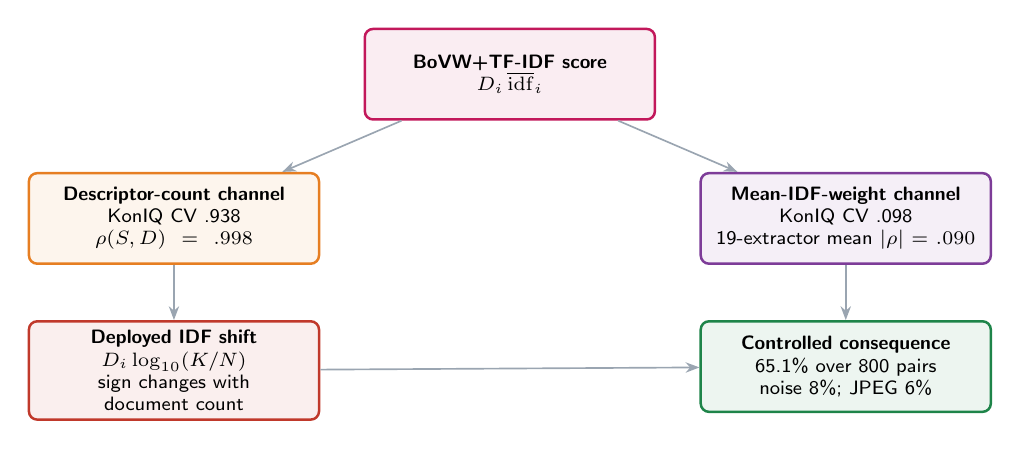
\begin{tikzpicture}[
  box/.style={rectangle,rounded corners=3pt,minimum height=1.15cm,
    text width=3.45cm,align=center,font=\sffamily\scriptsize,
    draw=#1,fill=#1!8,line width=.9pt},
  arr/.style={-{Stealth[length=5pt]},semithick,rulegray}]
\node[box=catbovw] (score) {\textbf{BoVW+TF-IDF score}\\$D_i\,\overline{\mathrm{idf}}_i$};
\node[box=accentorange,below left=.65cm and .55cm of score] (count)
 {\textbf{Descriptor-count channel}\\KonIQ CV .938\\$\rho(S,D)=.998$};
\node[box=accentpurple,below right=.65cm and .55cm of score] (rare)
 {\textbf{Mean-IDF-weight channel}\\KonIQ CV .098\\19-extractor mean $|\rho|=.090$};
\node[box=accentred,below=.7cm of count] (dep)
 {\textbf{Deployed IDF shift}\\$D_i\log_{10}(K/N)$\\sign changes with document count};
\node[box=accentgreen,below=.7cm of rare] (test)
 {\textbf{Controlled consequence}\\65.1\% over 800 pairs\\noise 8\%; JPEG 6\%};
\draw[arr] (score)--(count); \draw[arr] (score)--(rare);
\draw[arr] (count)--(dep); \draw[arr] (rare)--(test);
\draw[arr] (dep)--(test);
\end{tikzpicture}
\caption{Measured mechanism. The factorization identifies two channels; the
data determine their relative variation and connect count dominance to the
controlled-degradation failures.}
\label{fig:mechanism}
\end{figure}

On KonIQ-10k, the coefficient of variation is .938 for $D_i$ and .098 for mean
IDF weight. The canonical score consequently correlates .998 with descriptor
count. Its association with human scores is statistically equivalent, within
the operational $\pm.02$ margin, to that of keypoint density:
$\rho^{*}=.447$ for both, with score-to-keypoint correlation .998. Steiger's
$Z=.199$ is below the Bonferroni-corrected critical value of 3.95, and both
one-sided equivalence tests reject. KADID gives the same association-level
result under reference-block resampling: .125 for canonical BoVW and .123 for
keypoint density, paired difference $+.0024$, 95\% CI
$[-.0019,+.0084]$. This is equivalence of measured MOS/DMOS association, not
identity of the scores or constructs. The deployed formulation is almost exactly the sign-reversed
count on the large databases ($-.9999$ on KonIQ, $-.9998$ on KADID and
$-.9947$ on CLIVE). In the deployment regime its own descriptor count remains
dominant, $\rho(S_{\mathrm{dep}},D)=+.994$.

Replacing SIFT with 19 convolutional extractors does not raise the external
ceiling. Their mean $|\rho|$ is .090 on KonIQ and .112 on CLIVE, with no value
above .238 on either database; KADID ranges from .156 to .418. Fixed spatial
feature maps remove per-image count variation on the image databases, leaving
the rarity channel measured by the ablation. On broadcast segments, however,
the upstream key-frame selector varies the number of retained frames, so it
reintroduces count variation: across the 19 variants,
$\rho(S,D)=+.981$ to $+.997$. These results explain why exchanging the
extractor changes individual choices without making the ordering a better
predictor of quality. The explanation is limited to the evaluated vocabulary,
normalization and extraction regimes.

Simple normalization does not repair the mechanism. Dividing by descriptor
count exposes the weak mean-IDF-weight channel already measured by the ablation. Dividing
by frame count is also mismatched to the deployed operation because its internal
key-frame selector makes descriptor count nearly independent of duration. On the
42 clusters, frame normalization changes the uncalibrated DOVER two-branch-sum
output only from 47.4\% to 50.6\% and induces an inverse duration association
($\rho=-.52$). Full normalization and pooling results are in Tables~S6 and S9.

\subsection{External validation and screening}\label{sec:screen_results}

Within-reference KADID sensitivity separates the deployed operation from
specialized quality methods. Its mean direction-aligned correlation is $-.077$
(95\% CI $[-.124,-.030]$), with only 5 of 25 types above .50. LIQE,
QualiCLIP and CLIP-IQA$+$ reach .807, .849 and .808, respectively, each with 22
types above .50. Most remaining NR-IQA candidates also respond broadly, with
means from .607 to .733.

Table~\ref{tab:screening} applies the same complete-case rule to every method.
Released-weight exposure is visible because an in-database correlation is not a
generalization result. The generalization column reports the lowest signed
$\rho^{*}$ over every unseen database, rather than using an absolute value that
could hide inversion.

\begin{table}[!ht]
\centering
\caption{Complete-case method screening. Sensitivity reports the within-reference
mean and number of KADID types above .50. Generalization is the lowest signed
$\rho^{*}$ over all unseen databases. Floor is normalized agreement with Q-Align
on the common 42 clusters and its topic-block lower bound (L). Sup.: K =
KonIQ-10k opinion training; L = LIVE; OU = opinion-unaware; -- = no opinion
training; M = multi-database mixture. Q-Align is a reference, not a candidate.}
\label{tab:screening}
\scriptsize
\setlength{\tabcolsep}{1.7pt}
\renewcommand{\arraystretch}{1.08}
\begin{tabular}{@{}lcccccc@{}}
\toprule
\rowcolor{headerblue}
\hd{Method} & \hd{Sup.} & \hd{Pol.} & \hd{Sensitivity} &
\hd{Lowest unseen $\rho^{*}$} & \hd{Floor; L} & \hd{Eligible} \\
\midrule
\rowcolor{accentgreen!15}\textbf{LIQE} & K & \polup & .807; 22 & .723 & .551; .284 & \textbf{yes} \\
\rowcolor{accentgreen!15}\textbf{QualiCLIP} & OU & \polup & .849; 22 & .665 & .371; .143 & \textbf{yes} \\
\rowcolor{accentgreen!15}\textbf{CLIP-IQA$+$} & K & \polup & .808; 22 & .654 & .236; .034 & \textbf{yes} \\
\midrule
TOPIQ & K & \polup & .721; 20 & .511 & .506; .289 & no \\
\rowcolor{rowlight}MUSIQ & K & \polup & .733; 20 & .556 & .551; .297 & no \\
DBCNN & K & \polup & .668; 19 & .484 & .461; .274 & no \\
\rowcolor{rowlight}HyperIQA & K & \polup & .673; 19 & .462 & .371; .122 & no \\
NIQE & OU & \poldown & .607; 19 & .368 & .281; .012 & no \\
\rowcolor{rowlight}BRISQUE & L & \poldown & .657; 19 & .236 & .371; .136 & no \\
CLIP-IQA & OU & \polup & .645; 20 & .501 & .371; .045 & no \\
\rowcolor{catbovw!12}SIFT+BoVW (deployed) & -- & \polup & $-.077$; 5 & $-.445$ & .056; $-.308$ & no \\
\midrule
\rowcolor{rowlight}Q-Align & M & \polup & .880; 23 & -- & -- & reference \\
\bottomrule
\end{tabular}
\end{table}

Three methods are eligible: LIQE, QualiCLIP and CLIP-IQA$+$. This is an
eligibility set, not a ranking. QualiCLIP has the largest sensitivity mean,
whereas LIQE has the largest generalization margin. The set is unchanged when
the generalization threshold varies from .60 to .65 or the sensitivity coverage
cut varies from 12 to 22 types (Table~S10); at .55 MUSIQ is added, and at .70
only LIQE remains. ARNIQA and TReS are reported on completed axes only, so
neither enters this complete-case claim.

The database-level values show why the universal unseen-database clause matters.
LIQE obtains $\rho^{*}=.723$ on KADID and .865 on CLIVE; QualiCLIP obtains .665
and .757; CLIP-IQA$+$ obtains .654 and .805. TOPIQ and MUSIQ are strong on the
unseen authentic database (.811 and .789) but fall to .511 and .556 on KADID.
DBCNN and HyperIQA similarly fall from .756 and .750 on CLIVE to .484 and .462
on KADID. An existential rule would admit methods whose favourable authentic
result masks failure under controlled synthetic distortion. Conversely, the
three eligible methods pass the floor with overlapping topic-block intervals,
so the small in-domain sample cannot order them.

The floor axis illustrates that limitation directly. LIQE agrees with Q-Align
on 32 of 42 clusters ($\kappa_{\mathrm{uniform}}=.551$, 95\% CI
$[.284,.786]$); QualiCLIP agrees on 28 ($.371$, $[.143,.597]$); and
CLIP-IQA$+$ on 25 ($.236$, $[.034,.435]$). The deployed operation agrees on 21,
only 1.3 decisions above the uniform expectation, and its normalized interval
crosses chance ($.056$, $[-.308,.412]$). The candidates pass the floor, but the
broadly overlapping intervals do not support pairwise ordering. Results on the
15 human-annotated redundancy clusters are retained in Tables~S7--S8 rather than
mixed with the operational 42-cluster set.

The full P.1401 triad and database-level correlations are in Tables~S4 and S15.
The latter reports training-database contrasts descriptively, because database,
content, architecture and objective are not matched. Conditioning on detectable
keypoint density strongly attenuates the BoVW score but is not interpreted as a
causal partition of ``content density'' (Table~S16). Cost is also secondary to
eligibility: in the common environment the deployed operation takes 182~s per
cluster and LIQE 1.9~s (Table~S14).

\subsection{Constructed broadcast degradation}\label{sec:constructed_results}

Table~\ref{tab:constructed} removes the reference model from the decision: each
pair contains the same content before and after a known degradation. The
deployed operation is correct on 65.1\% of 800 pairs. LIQE reaches 99.5\%; the
paired difference is $+34.4$ percentage points, segment-block 95\% CI
$[+31.1,+37.7]$. Every evaluated NR-IQA candidate exceeds the deployed score.

\begin{table}[!ht]
\centering
\caption{Strict accuracy (\%) on 800 unmodified--degraded broadcast pairs: 20
segments, eight types and five levels. The unmodified member is the
construction-defined higher-fidelity signal; values below the 50\% chance floor
are systematic inversions. Ties remain in the denominator.}
\label{tab:constructed}
\scriptsize
\setlength{\tabcolsep}{1.9pt}
\begin{tabular}{@{}lccccccccc@{}}
\toprule
\textbf{Method} & \textbf{dark} & \textbf{motion} & \textbf{blur} & \textbf{H.264}
& \textbf{rescale} & \textbf{satur.} & \textbf{noise} & \textbf{JPEG} & \textbf{mean} \\
\midrule
\rowcolor{catbovw!12}SIFT+BoVW (deployed) & 100 & 100 & 90 & 90 & 88 &
\textcolor{accentred}{\textbf{39}} & \textcolor{accentred}{\textbf{8}} &
\textcolor{accentred}{\textbf{6}} & \textbf{65.1} \\
\midrule
LIQE & 97 & 100 & 100 & 100 & 100 & 100 & 99 & 100 & \textbf{99.5} \\
TOPIQ & 93 & 100 & 100 & 100 & 100 & 93 & 100 & 100 & 98.2 \\
MUSIQ & 93 & 100 & 100 & 100 & 100 & 86 & 100 & 100 & 97.4 \\
QualiCLIP & 99 & 100 & 95 & 100 & 96 & 76 & 96 & 71 & 91.6 \\
ARNIQA & 91 & 100 & 99 & 98 & 100 & 61 & 82 & 98 & 91.1 \\
DBCNN & 84 & 97 & 92 & 97 & 95 & 92 & 85 & 81 & 90.4 \\
NIQE & 100 & 100 & 98 & 97 & 98 & \textcolor{accentred}{\textbf{0}} & 100 & 96 & 86.1 \\
CLIP-IQA$+$ & 76 & 99 & 79 & 100 & 91 & 87 & 84 & 64 & 85.0 \\
HyperIQA & 47 & 100 & 100 & 100 & 100 & \textcolor{accentred}{\textbf{30}} & 100 & 100 & 84.6 \\
CLIP-IQA & 58 & 100 & 83 & 100 & 92 & 91 & 55 & 76 & 81.9 \\
BRISQUE & 100 & 100 & 100 & 99 & 100 & \textcolor{accentred}{\textbf{0}} & 67 & 80 & 80.8 \\
\bottomrule
\end{tabular}
\end{table}

No method ties on these pairs. Excluding darkening and desaturation leaves 600
comparisons and does not repair the deployed operation: its accuracy is 63.7\%,
whereas LIQE reaches 99.8\% and Q-Align 100\% (Table~S12). The main diagnosis
therefore does not depend on treating those two transformations as universally
worse in human perception.

The average conceals the diagnostic result. SIFT+BoVW is at or above 88\% on
five types but selects the degraded copy in 92\% of white-noise pairs and 94\%
of JPEG pairs. Within segment, its score increases with severity for noise
($\rho=+.720$, CI $[+.455,+.925]$) and JPEG ($+.640$, CI
$[+.395,+.850]$). The mechanism is directly visible in the saved descriptor
counts. The degraded copy has more descriptors in 92\% of noise pairs (mean
change $+469$) and 95\% of JPEG pairs (mean change $+289$), with mean noise
count increasing at every severity level. These measurements are consistent
with noise and blocking creating detectable extrema that increase the count
channel in Eq.~\ref{eq:factor}; structure-removing distortions instead happen
to move count in the direction of fidelity. The score is therefore responsive,
but not consistently to quality (Table~S12).

Q-Align is correct on 98.2\% of these pairs (95\% CI $[97.2,99.1]$), which
supports its technical-degradation competence on this broadcast content. It
does not validate compositional preference. The exact downstream DOVER-T output
reaches 97.6\% ($[96.1,99.0]$), or 99.8\% ($[99.5,100]$) without darkening and
desaturation; neither result is a human judgment. The 19
extractor substitutions average 44.9\% (CI $[41.0,48.9]$) and remain dominated
by their descriptor count, corroborating the mechanism while refuting the
recorded prediction that fixed feature maps would force chance performance.
The full prediction and overlay audits are in Table~S12.

\subsection{Pipeline substitution}\label{sec:e2e}

LIQE is used for the direct operation substitution because it has the largest
generalization margin among the three eligible methods and near-ceiling accuracy
on the constructed pairs. With the same ten uniformly spaced frames and mean
pooling, SIFT+BoVW and LIQE still differ in 16 of 42 clusters. The LIQE--SIFT
DOVER-T contrast is $+27.1$ range points (topic CI $[5.6,47.8]$; hierarchical
$[2.4,52.5]$) and $+.0074$ raw, with both intervals positive (Table~S11).
Table~\ref{tab:e2e} reports the complete-operation comparison and all eligible
methods; screening does not rank them.

\begin{table}[!ht]
\centering
\caption{Model-reference output over the 42 operational redundancy clusters.
Changed counts representatives differing from the deployed operation. DOVER-T
is the raw DOVER technical branch and is not used in screening; Q-Align defines
the in-domain screening floor. Both outputs use the global-achievable-range
estimand in Eq.~\ref{eq:globalrange}; Max is the percentage of clusters in which
the selected representative has the highest DOVER-T score.}
\label{tab:e2e}
\small
\setlength{\tabcolsep}{5pt}
\renewcommand{\arraystretch}{1.08}
\begin{tabular}{@{}lcrrr@{}}
\toprule
\rowcolor{headerblue}
\hd{Quality operation} & \hd{Changed} & \hd{DOVER-T} & \hd{Max} & \hd{Q-Align} \\
\midrule
\rowcolor{catbovw!12}SIFT+BoVW & --- & 50.5\% & 54.8\% & 48.6\% \\
\rowcolor{accentgreen!15}\textbf{LIQE} & \textbf{22/42} & \textbf{76.0\%} & 59.5\% & 90.2\% \\
QualiCLIP & 19/42 & 71.9\% & 59.5\% & 80.6\% \\
\rowcolor{rowlight}CLIP-IQA$+$ & 22/42 & 70.7\% & 50.0\% & 74.3\% \\
\bottomrule
\end{tabular}
\end{table}

Replacing the deployed visual-quality operation with the LIQE-based operation
changes 22 of 42 representatives. On the primary DOVER technical branch, the
global-achievable-range point estimate rises from 50.5\% to 76.0\%, a paired
increase of $+25.5$ points. Its topic-block interval is $[-12.1,+54.9]$ and its
hierarchical interval is $[-17.2,+59.6]$; neither confirms a population-level
effect. The raw branch-score difference is $+.0069$ (topic-block
$[-.0028,+.0178]$; hierarchical $[-.0041,+.0197]$), while mean per-cluster
position and selected-maximum rate increase by 7.2 and 4.8 points, respectively.

No cluster has zero DOVER-T range. Excluding the smallest 10\% or 25\% of ranges
gives global-range differences of $+25.9$ and $+28.1$ points, so the positive
point estimate is not generated solely by near-zero ranges. As a construct
sensitivity analysis, the uncalibrated sum of DOVER's technical and aesthetic
branches reproduces the earlier $+30.3$-point contrast, but that sum is neither
the official standardized fused score nor a purely technical measure
(Table~S11).

The two model references have positive point estimates for the substitution but not on
the ordering within the eligible set. That disagreement, together with
overlapping intervals, is why the study reports eligibility rather than a
winner. More importantly, neither column measures human preference for the
composed summary. The supported end-to-end conclusion is that the operation
substitution materially changes the selected evidence; the model-reference
output effects are positive but imprecise, and improved viewer experience
remains untested.

\section{Discussion and limitations}\label{sec:discussion}

The evidence converges on a localized diagnosis. The canonical score and
keypoint density have statistically equivalent MOS/DMOS associations within the
operational $\pm.02$ margin on KADID and KonIQ; the implementation adds a
count-proportional term whose sign changes with collection size; and all 19
extractor substitutions remain bounded while tracking their descriptor counts.
The constructed pairs reveal the consequence: noise and JPEG artefacts add
detectable structure and reverse the ordering. A proxy can therefore appear
competent on selected distortions while responding to the wrong construct.

This is not an impossibility theorem for all BoVW uses. Equation~\ref{eq:factor}
identifies the two channels in this aggregation but does not prove that count or
mean IDF weight can never correlate with quality under another detector,
vocabulary, normalization or distribution. The empirical result is that count
dominates the evaluated configurations and that neither the measured
mean-IDF-weight channel nor the extractor substitutions recover a reliable
quality ordering.

The practical implication is to replace the operation rather than normalize it
by segment length or insert a newer retrieval descriptor. LIQE, QualiCLIP and
CLIP-IQA$+$ meet the common rule and run substantially faster than the deployed
path, but the rule does not rank them. The LIQE substitution demonstrates
propagation, not universal superiority. The complete operation changes 22
decisions; the matched control changes 16 and retains positive DOVER-T intervals.
Thus scorer identity matters, but internal operation choices also contribute.
DOVER does not isolate temporal modelling because architecture and training also
differ.

The summarization claim is conditional. Cluster membership means that the
pipeline treats segments as redundant alternatives; it does not establish
identical completeness, narrative utility, audio quality or semantic relevance.
A technically cleaner representative can omit context or carry worse audio, so
visual quality remains a tie-breaker rather than an objective for the summary as
a whole. A future human study should separately ask which segment has better
technical visual quality and which is preferred in the composed summary.

The references also have bounded roles. KADID and the broadcast construction
test responses to degradation, not preference between distinct recordings.
Q-Align's 98.2\% constructed-pair accuracy supports technical-degradation
screening; the exact DOVER technical output used downstream reaches 97.6\% on
the same pairs. This validates its response to the constructed technical
changes, not its use as human ground truth or a compositional preference model.
The official standardized fusion and DOVER++ remain outside the analysis.

The application remains imprecise: 42 clusters are nested in only 19 topics,
and both DOVER-technical intervals cross zero. Positive raw, range and rank
point estimates, including after removing small-range clusters, do not confirm a
population-level output effect. Coverage is also incomplete: ARNIQA and TReS are
partial, MANIQA is absent, and later models may change the eligible set.

Finally, the auxiliary analyses are descriptive. KonIQ--CLIVE--KADID contrasts
change content, capture, score distributions and model exposure together, while
conditioning on keypoint density may remove legitimate quality signal. Tables
S15 and S16 retain those diagnostics; the main conclusion rests on the exact
factorization, dependency-aware external measurements, constructed pairs,
matched-input control and controlled operation substitution.

\section{Conclusion}\label{sec:conclusion}

This study audited the operation implementing a human-grounded visual-quality
criterion in one multi-video summarization pipeline. The deployed
SIFT+BoVW+TF-IDF score factors into descriptor count and mean IDF weight. Under the
evaluated vocabularies, normalizations and extractors, descriptor count dominates:
the canonical score and keypoint density have statistically equivalent
MOS/DMOS associations within the operational $\pm.02$ margin on KADID and
KonIQ, whereas the deployed formulation produces a near-exact sign-reversed
count ordering in the large-database regime. In the broadcast domain,
the deployed score tracks its own descriptor count at $+.994$ and remains
bounded when SIFT is replaced by 19 convolutional extractors.

The mechanism predicts a consequential failure. Across 800 unmodified--degraded
broadcast pairs, the deployed operation selects the construction-defined
higher-fidelity member in 65.1\% of decisions and systematically prefers
white-noise and JPEG-degraded copies. LIQE reaches 99.5\%. A dependency-aware
screening rule retains LIQE, QualiCLIP and CLIP-IQA$+$; substituting the complete
visual-quality operation with a LIQE-based operation, while holding every other
pipeline stage fixed, changes 22 of 42 selected segments. The DOVER
technical-branch global-range point estimate increases by 25.5 percentage
points, but both topic-block and hierarchical intervals cross zero, so no
population-level output effect is confirmed.

The supported conclusion is therefore specific: the audited operation is not a
reliable perceptual-quality proxy in the tested regimes, and eligible NR-IQA
replacements materially alter its decisions. With frames and pooling matched,
SIFT+BoVW and LIQE still disagree in 16 of 42 clusters; 13 of these disagreements
overlap the 22 changes in the complete-operation comparison. The study does not establish that
all BoVW formulations fail, that redundancy clusters contain semantically
identical alternatives, or that viewers prefer the modified summaries. Human
pairwise evaluation and broader video-native quality assessment remain the next
tests needed to connect technical visual quality to compositional value.


\section*{Statements and Declarations}

\paragraph{Competing interests}
The authors declare that they have no competing financial or non-financial
interests that could have appeared to influence the work reported in this
article.

\paragraph{Data availability}
KADID-10k, KonIQ-10k and LIVE In the Wild are public. Supplementary Tables
S1--S16 and a reproducibility archive accompany the submission. Before final
acceptance, scripts, derived scores, clusters, annotations, seeds and latency
results will receive a versioned Zenodo DOI. The HSMVideoSumm news videos remain
subject to their original redistribution terms; only permitted derivatives will
be archived. The submission archive includes a Git bundle that makes the full
registered-prediction commit independently verifiable.

\paragraph{Code availability}
Analysis scripts and machine-readable results accompany the submission and will
be released at \url{https://github.com/Prism411/quality-benchmark} with the
versioned archive.

\paragraph{Author contributions}
%% TODO: adjust to the final author list.
J.\,L.\,S.\,G. designed and implemented the evaluation protocol, ran the
experiments and wrote the manuscript. R.\,G. supervised the research, defined
the problem framing within the multi-video summarization pipeline and revised
the manuscript. Both authors read and approved the final version.

\paragraph{Ethics approval}
Not applicable. The study uses publicly broadcast news material and three
publicly released image quality databases; no new human subject data were
collected.

\bibliography{references}
\end{document}
